\documentclass[10pt]{article}
\usepackage{icmlko}

\icmlmeta{IP 파운데이션 월드모델}{99}{받으면 잃는다}{대상 넷에 설명문과 표지를 붙였더니 --- 팝업이 자기 설명문을 받는 순간 남이 준 $+$0.0183이 $-$0.0013으로 무너졌다}

\begin{document}

\twocolumn[
\icmlheader

\begin{abstract}
노트 96--98은 전부 \emph{출처} 쪽 이야기였다. 팝업이 얻는 것은 $+$0.022에서
멈췄고 그 천장을 우회하는 길은 하나뿐이었다 --- \textbf{대상 자신이 축을 갖는
것.} 캐시와 인터넷에서 캤다. \textbf{팝업} 레코드의 기획 개념문 68/75(91\%) ·
\textbf{도서} 알라딘 상품 페이지 243건을 새로 받아 책소개 243/243 · \textbf{펀딩}
텀블벅 캐시에서 소개문 400/400과 표지 400/400 · \textbf{아이돌} 아이튠즈에서
앨범 표지 61/81. 표지는 641장을 새로 받아 실패 0건. 이제 \textbf{설명문 아홉
도메인 13,118건 · 표지 여덟 도메인 12,329장}이다. \textbf{그런데 결과가
정반대다.} 출처 여섯만 받을 때 팝업은 $+$0.0183인데, \textbf{아홉 전부(대상
셋 포함)로 넓히면 $+$0.0036}이고 \textbf{대상 셋만 주면 $-$0.0026}이다. 표지도
같다(다섯 $+$0.0220 $\to$ 여덟 $+$0.0098). 하나씩 더해 갈랐다 --- 도서가 받아도
팝업은 $+$0.0187, 펀딩이 받아도 $+$0.0190으로 \textbf{꿈쩍 안 한다}. 그런데
\textbf{팝업 자신이 받는 순간 $+$0.0036}으로 떨어지고, 출처 여섯에 팝업만
더하면 \textbf{$-$0.0013}이다. \textbf{받는 벌이 남이 준 이득과 거의 정확히
같다.} 노트 98이 관측한 ``받은 도메인은 나빠진다''가 팝업에도 그대로 걸린다 ---
\textbf{팝업이 이득을 본 이유는 안 받았기 때문이었다.} 제품에 곧장 붙는 결론이
있다 --- \textbf{도구는 팝업의 기획 개념문을 축으로 쓰면 안 된다.}
\end{abstract}
]

\begin{figure*}[t]
\centering
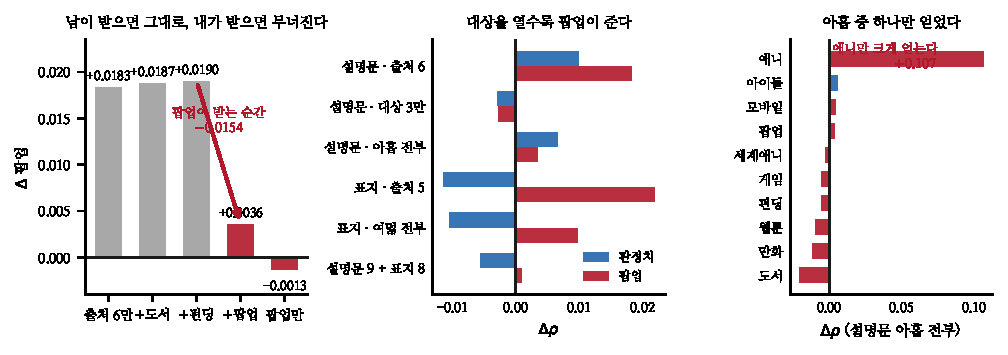
\includegraphics[width=\textwidth]{figs/rv.pdf}
\caption{왼쪽 --- 남이 받으면 그대로, 내가 받으면 무너진다. 가운데 --- 대상을
열수록 팝업이 준다. 오른쪽 --- 아홉 중 하나만 얻었다.}
\end{figure*}

\section{대상 넷을 열었다}

노트 96 · 97 · 98의 한계 항목에 세 번 연속 실린 것이 하나 있다 --- ``팝업 ·
아이돌 · 도서 · 펀딩에는 축이 없다.'' 넷 다 찾았다.

\begin{table}[t]
\centering\tsize
\caption{대상 넷에서 캔 것. 굵은 것이 이번에 새로 받은 것.}
\begin{tabular}{llrr}
\toprule
& 출처 & 설명문 & 표지 \\
\midrule
팝업 & 레코드 기획 개념문 & 91\% & --- \\
도서 & \textbf{알라딘 상품 페이지} & \textbf{100\%} & 99\% \\
펀딩 & 텀블벅 캐시 & 100\% & \textbf{100\%} \\
아이돌 & \textbf{아이튠즈 앨범} & --- & \textbf{75\%} \\
\bottomrule
\end{tabular}
\end{table}

도서는 알라딘 상품 페이지 243건을 새로 받아 \texttt{og:description} 에서
책소개를 뽑았고(243/243), 표지는 641장을 새로 받았다(실패 0건). 아이돌은
아이튠즈 검색 API 로 그룹명을 찾아 앨범 표지를 받았다(61/81).

\begin{table}[t]
\centering\tsize
\caption{지금 가진 것. 노트 95에서 다섯이었다.}
\begin{tabular}{lrr}
\toprule
& 도메인 & 건수 \\
\midrule
설명문 & \textbf{9} & \textbf{13,118} \\
표지 & \textbf{8} & \textbf{12,329} \\
\bottomrule
\end{tabular}
\end{table}

\section{그런데 결과가 정반대다}

\begin{table}[t]
\centering\tsize
\caption{설명문 임베딩 첫 성분과 표지 첫 주성분을 고유 축으로.}
\begin{tabular}{lrr}
\toprule
& $\Delta$판정치 & $\Delta$팝업 \\
\midrule
설명문 · 출처 6(노트 96) & $+$0.0099 & \textbf{$+$0.0183} \\
설명문 · 대상 3만 & $-$0.0028 & $-$0.0026 \\
설명문 · \textbf{아홉 전부} & $+$0.0066 & \textbf{$+$0.0036} \\
\midrule
표지 · 출처 5(노트 97) & $-$0.0113 & \textbf{$+$0.0220} \\
표지 · \textbf{여덟 전부} & $-$0.0103 & \textbf{$+$0.0098} \\
\midrule
설명문 9 $+$ 표지 8 & $-$0.0054 & $+$0.0010 \\
\bottomrule
\end{tabular}
\end{table}

\claimx{대상 쪽을 열면 \textbf{나빠진다.} 데이터를 세 배로 늘리고 도메인을
여섯에서 아홉으로 넓혔는데 팝업 이득이 $+$0.0183에서 $+$0.0036으로 준다.
설명문과 표지를 다 넣으면 $+$0.0010, 사실상 0이다.}{설명문 코퍼스를 아홉
도메인으로 다시 적합했으므로 노트 96의 $+$0.0222와 여기 $+$0.0183은 같은
축이 아니다. 코퍼스가 바뀌면 SVD 성분도 바뀐다.}

\section{받는 벌을 갈랐다}

출처 여섯은 고정하고 \emph{대상}을 하나씩 더 받게 했다.

\begin{table}[t]
\centering\tsize
\caption{누가 받느냐만 바꾼다.}
\begin{tabular}{lrr}
\toprule
받는 쪽 & $\Delta$판정치 & $\Delta$팝업 \\
\midrule
출처 6만 & $+$0.0099 & \textbf{$+$0.0183} \\
$+$도서 & $+$0.0077 & $+$0.0187 \\
$+$펀딩 & $+$0.0083 & \textbf{$+$0.0190} \\
\midrule
$+$\textbf{팝업} & $+$0.0066 & \textbf{$+$0.0036} \\
출처 6 $+$ 팝업만 & $+$0.0074 & \textbf{$-$0.0013} \\
\bottomrule
\end{tabular}
\end{table}

\claimx{\textbf{받는 벌이 남이 준 이득과 거의 정확히 같다.} 도서 · 펀딩이
받아도 팝업은 $+$0.0187 · $+$0.0190으로 꿈쩍 안 하는데, 팝업 자신이 받으면
$-$0.0154가 깎여 $+$0.0036이 되고, 출처 여섯에 팝업만 더하면 $-$0.0013으로
\textbf{이득이 전부 사라진다.}}{팝업 설명문 덮개율이 91\%라 결측 표시자
한 칸이 더 붙는다. 축이 둘 늘어난 셈이므로 희석이 다른 도메인보다 크다.}

\begin{quote}\fontsize{9.5}{11.5}\selectfont
\textbf{노트 96--98의 이야기가 여기서 닫힌다.} 노트 96은 ``없는 축이 돕는다''고
했고 노트 98은 ``받은 도메인은 평균 $-$0.0241''을 관측했다. 두 문장은 같은
법칙의 앞뒤였다 --- \textbf{축을 받으면 자기 인자 공간이 희석돼 잃고, 남이
받으면 그 출처가 좋아져 얻는다.} 팝업이 넉 노트에 걸쳐 유일하게 이득을 본
이유는 팝업이 좋아서가 아니라 \textbf{팝업만 안 받았기 때문}이었다.
\end{quote}

\section{아홉 중 하나만 얻었다}

\begin{table}[t]
\centering\tsize
\caption{설명문을 아홉 도메인에 다 넣었을 때 대상별.}
\begin{tabular}{llrr}
\toprule
& & 현행 & $\Delta$ \\
\midrule
\textbf{애니} & 받음 & $+$0.274 & \textbf{$+$0.107} \\
아이돌 & 안 받음 & $+$0.473 & $+$0.006 \\
모바일 & 받음 & $+$0.617 & $+$0.004 \\
팝업 & 받음 & $+$0.450 & $+$0.004 \\
세계애니 & 받음 & $+$0.418 & $-$0.002 \\
게임 & 받음 & $+$0.397 & $-$0.005 \\
펀딩 & 받음 & $+$0.214 & $-$0.005 \\
웹툰 & 받음 & $+$0.483 & $-$0.010 \\
만화 & 받음 & $+$0.473 & $-$0.012 \\
도서 & 받음 & $+$0.239 & $-$0.020 \\
\bottomrule
\end{tabular}
\end{table}

\claimx{설명문 축이 실제로 구하는 도메인은 \textbf{애니 하나}다($+$0.107).
나머지 여덟은 $\pm$0.02 안이고 대부분 음수다.}{애니가 왜 다른지 모른다.
노트 75가 애니의 배선을 고쳤고 굿즈 규모 슬롯이 0\%인 도메인인데, 슬롯이 더
빈 게임($-$0.005)은 안 얻는다. 관측 축 수로도 표본으로도 안 갈린다.}

\section{제품에 붙는 결론}

\begin{quote}\fontsize{9.5}{11.5}\selectfont
\texttt{state/score.py} 는 기획안 열 속성을 받아 과거 팝업 중 백분위를 낸다.
\textbf{여기에 기획 개념문을 축으로 더하면 안 된다.} 직관과 반대지만 측정이
분명하다 --- 팝업이 자기 설명문을 축으로 받으면 아홉 출처가 준 $+$0.0183이
$-$0.0013이 된다. 설명문은 \emph{출처 도메인}에서만 값을 한다.
\end{quote}

\section{채택 검정}

\begin{table}[t]
\centering\tsize
\caption{설명문 · 출처 여섯. 씨앗 넷 · 붓스트랩 100회.}
\begin{tabular}{lrl}
\toprule
& $\Delta$ & 95\% 구간 \\
\midrule
판정치 & $+$0.0099 & $[-0.0196, +0.0180]$ \quad 보류 4/4 \\
팝업 & $+$0.0183 & $[-0.0409, +0.0841]$ \quad 보류 4/4 \\
\bottomrule
\end{tabular}
\end{table}

\textbf{채택하지 않는다.} 이 노트의 어느 설정도 문턱을 못 넘는다.

\section{한계}

\begin{itemize}[leftmargin=1.1em,itemsep=0.15em]
\item 설명문 SVD 를 아홉 도메인 코퍼스로 다시 적합했으므로 노트 96의 수치와
      직접 비교가 안 된다. 코퍼스가 바뀌면 성분이 바뀐다.
\item 팝업 설명문이 91\%라 결측 표시자가 한 칸 더 붙는다. ``받는 벌''의 일부는
      덮개율 탓일 수 있다 --- 100\%인 도서 · 펀딩은 벌이 없었다는 것이 반증이지만
      그 둘은 애초에 팝업 이득에 영향이 없었다.
\item 아이돌은 설명문을 못 구했고 표지도 75\%다. 팝업은 표지가 아예 없다.
\item ``애니만 얻는다''를 설명 못 한다.
\item 대상 쪽 축을 \emph{고유 축}으로만 넣었다. 공통 슬롯으로 넣는 설정은 안
      해 봤다.
\end{itemize}

\section{다음}

\begin{enumerate}[leftmargin=1.3em,itemsep=0.15em]
\item \textbf{희석을 없애고 다시 본다} --- 받는 벌이 ``인자 공간이 $k{=}2$로
      고정인데 축만 늘어서''라면, 받는 도메인만 $k{=}3$으로 올리면 벌이
      사라져야 한다. 이것이 받는 벌의 기제 검정이다.
\item \textbf{애니를 갈라 본다} --- 아홉 중 하나만 얻은 이유. 애니의 무엇이
      다른지 알면 어떤 도메인에 새 축을 붙일지 고를 수 있다.
\item 팝업 설명문을 축이 아니라 \textbf{라벨 보정}에 쓴다 --- 축으로는
      손해지만 다른 쓰임이 있을 수 있다.
\item 출처 도메인을 아홉 너머로. 노트 96의 셈은 여전히 미판정이다.
\end{enumerate}

\vspace{0.6em}
\hrule height 0.3pt
\vspace{0.5em}
{\footnotesize
\textbf{참고문헌}\\[0.3em]
Ben-David, S. et al. (2010). A theory of learning from different domains.
\emph{Machine Learning}, 79(1--2), 151--175.\\[0.15em]
Schoenemann, P. H. (1966). A generalized solution of the orthogonal Procrustes
problem. \emph{Psychometrika}, 31(1), 1--10.\\[0.15em]
Little, R. J. A., Rubin, D. B. (2019). \emph{Statistical Analysis with Missing
Data}, 3rd ed. Wiley.\\[0.15em]
Deerwester, S. et al. (1990). Indexing by latent semantic analysis.
\emph{JASIS}, 41(6), 391--407.\\[0.15em]
Efron, B., Tibshirani, R. J. (1993). \emph{An Introduction to the Bootstrap}.
Chapman \& Hall.
}

\end{document}
